\section*{Listen}
	\hspace{2cm}
	\rowcolors{1}{blue!10}{white}
	\begin{tabular}{|l l l|}
		\hline list.append(x) & list.extend(iterable) & list.remove(x)
		\\ list.clear() & list.index(x[, start[, end]]) $\to$ int & list.reverse()
		\\ list.copy() $\to$ list & list.insert(i, x) & list.sort(key=None, reverse=False)
		\\ list.count(x) $\to$ int & list.pop([i]) $\to$ object & 
		\\\hline
	\end{tabular}
	\vspace{0.5cm}
	\\\vspace{0.1cm}
%%%%%%%%%%%%%%%%%%%%%%%%%%%%%%%%%%%%%%%%%%%%%%%%%%
	\textbf{Erzeugen von Listen}
	\\
	\begin{minipage}[h]{10cm}
		\lstinputlisting{code/Listen/Listen_create.py}
	\end{minipage}
	\begin{minipage}[h]{8cm}
		\textcolor{red}{\textbf{Out:}} \\
		mylist = [1, 2, 3], alist = [4, 5, 6]
	\end{minipage}
%%%%%%%%%%%%%%%%%%%%%%%%%%%%%%%%%%%%%%%%%%%%%%%%%%
	\newpage
%%%%%%%%%%%%%%%%%%%%%%%%%%%%%%%%%%%%%%%%%%%%%%%%%%
	\hspace{-0.5cm}
	\textbf{Hinzufügen/Entfernen von Elementen}
	\\
	\begin{minipage}[h]{10cm}
		\lstinputlisting{code/Listen/Listen_add_delete.py}
	\end{minipage}
	\begin{minipage}[h]{8cm}
		\textcolor{red}{\textbf{Out:}}
		\\\#1 mylist = [1, 2, 33, 11, 22]
		\\\#2 mylist = [1, 2]
		\\\#3 mylist = []
	\end{minipage}
%%%%%%%%%%%%%%%%%%%%%%%%%%%%%%%%%%%%%%%%%%%%%%%%%%
	\vspace{0.5cm}
	\\\textbf{Indexierung/Slicing}\\
	slice = lst[start:end:step]
	'inklusiv' start bis 'exklusiv' end\\
	\begin{minipage}[h]{6cm}
		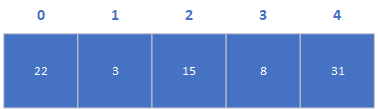
\includegraphics[width=6cm,align=t]{pics/Listen/indexing_pos.png}
	\end{minipage}
	\begin{minipage}[h]{6cm}
		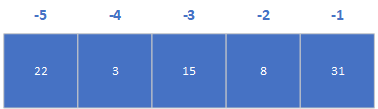
\includegraphics[width=6cm,align=t]{pics/Listen/indexing_neg.png}
	\end{minipage}
	\begin{minipage}[h]{6cm}
		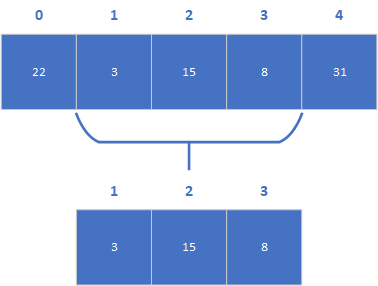
\includegraphics[width=6cm,align=t]{pics/Listen/slicing.png}
	\end{minipage}
	\\
	\begin{minipage}[h]{10cm}
		\lstinputlisting{code/Listen/Listen_slicing.py}
	\end{minipage}
	\begin{minipage}[h]{8cm}
		\textcolor{red}{\textbf{Out:}}
		\\mylist[::] = [22, 3, 15, 8, 31]
		\\mylist[1:4] = [3, 15, 8]
		\\mylist[::2] = [22, 15, 31]
		\\mylist.index(3) = 1
	\end{minipage}
%%%%%%%%%%%%%%%%%%%%%%%%%%%%%%%%%%%%%%%%%%%%%%%%%%
	\vspace{0.5cm}
	\\\textbf{Sortieren}
	\vspace{0.1cm}
	\\
	\begin{minipage}[h]{10cm}
		\lstinputlisting{code/Listen/Listen_sort.py}
	\end{minipage}
	\begin{minipage}[h]{8cm}
		\textcolor{red}{\textbf{Out:}}
		\\\#1 [2, 3, 3, 4, 5, 7]
		\\\#2 [7, 5, 4, 3, 3, 2]
		\\\#3 1
		\\\#4 ['GM', 'BMW', 'Tesla']
	\end{minipage}
